In this thesis, we have investigated the dimension of the inertial manifold
in the one\dmn\ \KSe\ and determined that the dimension is 8 for domain size $22$.
In order to reach this conclusion, we had to develop a number of
theoretical and numerical tools. Here, we summarize the contributions of
this thesis in two categories, theoretical and numerical contributions,
and discuss open future directions.


\section{Theoretical contributions}

In \refsect{sect:tang}, we define the projection operator from
full \statesp\ to the slice. Also, in \refsect{sect:sliceJac},
we give the precise relation between the
in-slice Jacobian and the Jacobian in the full \statesp. Therefore,
in-slice stability eigenvectors can be obtained easily from those
in the full \statesp.

% In \refsect{sect:fact}, we generalize the discrete factorization of
% evolution operator for group $C_n$ and $C_{nv}$, which serves as a
% reference for people who are investigating systems with a specific
% symmetry such as $C_3$, $C_{3v}$ and so on.

In \refsect{sect:ksO2}, we reduce the \On{2} symmetry by using the
fundamental domain and argue that defining the 1st mode slice
to have vanishing real part of the first Fourier mode will keep
the reflection rule unchanged in the slice.
Such a simplification can be adopted in other systems with
\On{2} symmetry too, such as \cGLe.

In \refsect{sect:ksdim}, we use three different numerical approaches, \ie,
local Floquet exponents, principal angles obtained by Floquet vectors, and expansion errors of
difference vectors in shadowing incidences, to estimate the dimension of
the inertial manifold in one\dmn\ \KSe. The results are consistent among
all these three approaches and with the previous research on covariant
Lyapunov vectors conducted on ergodic trajectories.

% \subsection{\CqcGLe}
% \label{sect:concl_cqcgl}
% In exploring potential generalizations of our methodology to other PDEs, we
% have focused on the \cqcGLe, with its rich spatiotemporal and solitonic
% phenomenology.
% Our main result, the discovery of ``exploding relative periodic orbits''
% region in the parameter space of this equation, does not fit easily
% into the main thrust of this thesis, and is thus not included here. The two
% completed papers on this topic (the second describes the numerical methods
% that had to be developed for this exploration), are currently awaiting
% collaborators' final approval prior to their submission:

% X. Ding and P. Cvitanovi{\'c},
% {\em Relative periodic orbit explosion in cubic-quintic complex
% {Ginzburg--Landau} equation}\rf{DingCvit16},
% and
% X. Ding  and , P. Cvitanovi{\'c} and S. H. Kang
% {\em Integration of a cubic-quintic complex {Ginzburg--Landau} exploding
% soliton}\rf{DingKang16}.


\section{Numerical contributions}

In \refchap{chap:ped},
we provide a detailed description of the \ped\ needed to calculate the stability
of \po s of a chaotic system. Its effectiveness and accuracy are
tested in the one\dmn\ \KSe\ in \refsect{sect:applic}.
The \texttt{C++}
implementation can be found at my GitHub repository
\href{https://github.com/dingxiong/research}
{github.com/dingxiong/research}.

This repository also contains the \texttt{C++} implementation of some
other algorithms that are frequently used in the study of chaotic systems,
such as GMRES\rf{Saad1986} to solve linear equation $Ax=b$ by Krylov
subspace iteration,
Levenberg-Marquardt algorithm\rf{levenberg44, Marquardt63},
inexact Newton backtracking method\rf{Simonis2006},
Newton-GMRES-Hookstep algorithm\rf{ChaKer12} to find (relative)
\po s, and the integrator for the one\dmn\ \KSe.

\section{Future work}

In this section, I list two potential directions for
the future research in this field.

\subsection{\Spt\ averages in \KSe}

We have gained valuable intuition about the geometrical structure of
the global attractor by the experience of working with these shadowing
cases in \refsect{sect:shadow}. We observe that the global attractor
has a very thin structure. Orbits can shadow the unstable manifold of
\EQV{2} and different orbits
can shadow each other. Experience with such shadowing incidences helps us
choose appropriate  \PoincSec s to capture the
transition rules between different subregions.
One is in a position to investigate the symbolic
dynamics of the system. Namely, one can try to partition the fundamental
domain into several subregions and figure out the transition rule
between different subregions. This transition rule, also called the symbolic
dynamics, helps us classify the over $60\,000$ pre/relative \po s by
their topological lengths. Then the \Fd\ \refeq{eq:sd}
could be accurately approximated by the shortest pre/relative
\po s.
If this is implemented, spatiotemporal averages could be obtained efficiently,
without longtime simulations.


\subsection{The dimensions of inertial manifolds of other systems}

We believe that the numerical techniques developed in \refchap{chap:im} can
be used to determine the dimensions of inertial manifolds for other nonlinear
dissipative dynamical systems. The previous studies\rf{YaTaGiChRa08,TaGiCh11,YaRa11},
based on \cLvs, have estimated the dimension of the inertial manifold of the
one\dmn\ \cGLe,
\[
  A_t = A + (1 + i\alpha)A_{xx} - (1 +i\beta)|A|^2A
  \,,
\]
where $A(x, t)$ is a complex field, and $\alpha$ and $\beta$ are real
parameters.  As shown in \reffig{fig:cGL_LargeL}, one\dmn\ \cGLe\
exhibits \spt\ chaos similar to the \KS\ \reffig{fig:KS_L100200}. We
believe (but have not carried out the requisite computations) that the
analysis based on \rpo s will also in this case determine the dimension
of inertial manifold. Similar to the one\dmn\ \KSe, this equation has a
spatial reflection symmetry $A(x,t)\to A(-x,t)$ and
\SOn{2}$\times$\SOn{2} spatial and phase translational symmetries
$A(x,t)\to e^{i\phi}A(x+\ell, t)$. Thus the symmetry-reduction techniques
discussed in \refsect{sec:symReduce} can also be applied here, and one
can restrict the analysis to a fundamental domain in a slice, as we did
in \refsect{sect:ksO2}. In two pubications not reported in detail in this
thesis\rf{DingKang16,DingCvit16}, we have constructed a ``minimal''
spatial domain and have determined a variety of \eqva, \reqva, and \rpo s
for this system. This sets the stage for application of methods discussed
in \refsect{sect:ksdim}, \ie, evaluation of local Floquet exponents,
principal angles among sets of Floquet vectors, and expansion errors of
difference vectors during close shadowing episodes, in order to estimate
dimensions of the inertial manifold in system of \cGL\ type.

\begin{figure}[h]
  \centering
  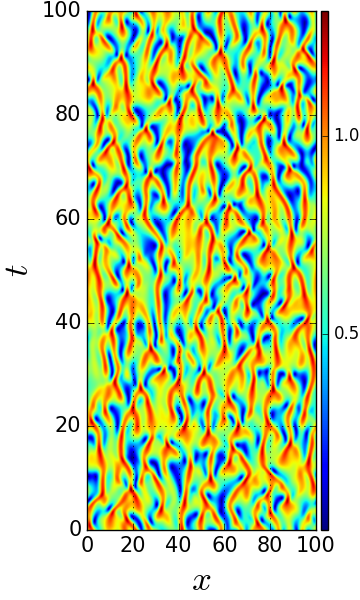
\includegraphics[height=0.35\textheight]{cGL_L100N256}
  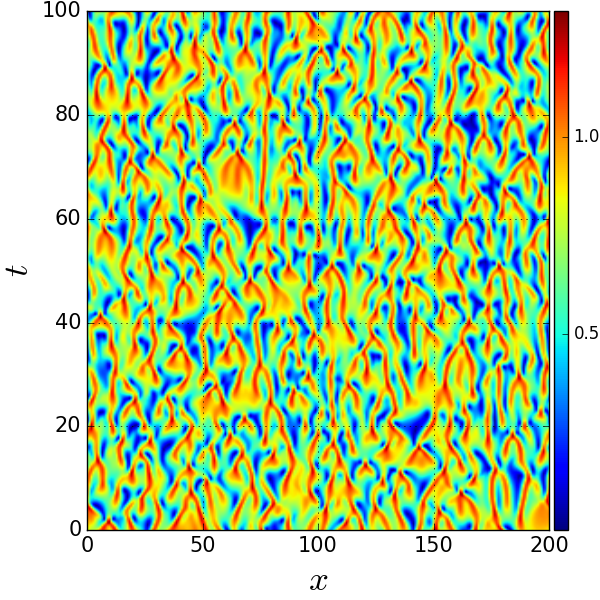
\includegraphics[height=0.35\textheight]{cGL_L200N256}
  \caption[\Spt\ plots of the one\dmn\ \cGLe\ for $L=100$ and $200$.]{
    \Spt\ plots  of \cGLe\ with $\alpha=2$ and $\beta=-2$ for two different domain sizes
    $L=100$ and $200$. The color represents the magnitude
    of the field $|A(x,t)|$. Random initial condition is used, with the initial transient
    discarded. Compare with \reffig{fig:KS_L100200}.
  }
  \label{fig:cGL_LargeL}
\end{figure}
